To calculate the magnetic field produced by a frustum permanent magnet, it is assumed ideal, with constant uniform magnetisation \(\mathbf{M}\) and a relative permeability \(\mu_r\) of unity. Under this assumption, a simplified version of the magnetic charge model outlined by \textcite{Furlani2001} can be applied to calculate the magnetic field \(\mathbf{B}\) at a point \(\mathbf{x}\), given by
\begin{equation}
\mathbf{B}\left(\mathbf{x}\right) = \frac{\mu_0}{4\pi} \oint_S \left( \mathbf{M} \cdot \hat{\mathbf{n}} \right) \frac{\mathbf{x} - \mathbf{x}'}{\left| \mathbf{x} - \mathbf{x}' \right| ^3} ds' \text{,}
\label{eqn:p3chargeModel}
\end{equation}
where \(\mu_0\) is the permeability of free space, \(\mathbf{M}\) is the magnetisation vector, \(\hat{\mathbf{n}}\) is the outward-facing unit normal vector of the magnet surface \(S\), \(\mathbf{x}'\) is a point on \(S\), and \(ds'\) is a surface element of \(S\).

This paper uses the field solution presented by the current authors \cite{OConnell2020a}, in which the magnet is deconstructed into each of its polygonal facets. Consider the rectangular pyramid frustum permanent magnet shown in Figure \ref{fig:p3myFrustum}. This is composed of two parallel rectangular surfaces and four trapezial surfaces joining the rectangles with symmetry in the \(XZ\) and \(YZ\) planes. One rectangular surface lies on the \(XY\)-plane, with the origin placed at the centre of the surface. The magnetic field is given by the sum of the field contributions from each of the rectangles \(\mathbf{B}_{\text{rect,}i}\) and trapezia \(\mathbf{B}_{\text{trap,}j}\),
\begin{align}
\mathbf{B} = \sum_{i=1}^2 \mathbf{B}_{\text{rect,}i} + \sum_{j=1}^4 \mathbf{B}_{\text{trap,}j} \text{.}
\end{align}
The following sections outline the methodology for calculating the field.
\begin{figure}
	\centering
	\def\lim{13}

\tdplotsetmaincoords{70}{45}
\begin{tikzpicture}[scale=0.115,tdplot_main_coords]

% Define coordinates:
\coordinate(ppb) at (15,20,-20);
\coordinate(pnb) at (15,-20,-20);
\coordinate(nnb) at (-15,-20,-20);
\coordinate(npb) at (-15,20,-20);
\coordinate(ppt) at (5,10,0);
\coordinate(pnt) at (5,-10,0);
\coordinate(nnt) at (-5,-10,0);
\coordinate(npt) at (-5,10,0);

% Fill in polygons:
\filldraw[fill=white] (ppt) -- (pnt) -- (nnt) -- (npt) -- cycle;
\filldraw[fill=white] (ppt) -- (ppb) -- (pnb) -- (pnt) -- cycle;
\filldraw[fill=white] (pnt) -- (nnt) -- (nnb) -- (pnb) -- cycle;

% Axes:
\draw[->] (0,0,0) -- (\lim,0,0);
\draw[->] (0,0,0) -- (0,\lim,0);
\draw[->] (0,0,0) -- (0,0,\lim);
\node(xaxis) at (\lim+2,0,0) {\(x\)};
\node(yaxis) at (0,\lim+2,0) {\(y\)};
\node(zaxis) at (0,0,\lim+2) {\(z\)};

\end{tikzpicture}
	\caption{A pyramid frustum created by joining two parallel rectangular surfaces with four quadrilateral surfaces. The rectangular surfaces are parallel to the \(XY\)-plane, with the origin at the centre of the top rectangular surface.}
	\label{fig:p3myFrustum}
\end{figure}

\subsection{Field solution for a magnetically charged trapezium}
Consider the magnetically charged trapezium depicted in Figure \ref{fig:p3trapezium} with surface charge \(\sigma = \mathbf{M} \cdot \hat{\mathbf{n}}\). It lies parallel to the \(\tilde{X}\tilde{Y}\)-plane with a \(\tilde{z}\)-coordinate of \(z'\) and the parallel edges being parallel to the \(\tilde{y}\)-axis. The magnetic field \(\mathbf{B}\left(\tilde{\mathbf{x}}\right) = \left[ B_{x}, B_{y}, B_{z} \right]\) due to this trapezium at the point \(\tilde{\mathbf{x}} = \left(\tilde{x}, \tilde{y}, \tilde{z}\right)\) is presented by the current authors \cite{OConnell2020a} and is given by
\begin{align}\label{eqn:p3fieldequation}
B_{\tilde{x}}\left(\tilde{\mathbf{x}}\right) &= \frac{\mu_0 \sigma}{4\pi} \sum_{p=1}^2 \sum_{q=1}^2 \Bigg[ \left( -1 \right) ^{p+q} \Bigg( \ln \left( T_{pq} \right) - \frac{m_p}{\sqrt{1+m_p^2}} \ln \left(S_{pq}\right) \Bigg) \Bigg] \nonumber \\
B_{\tilde{y}}\left(\tilde{\mathbf{x}}\right) &= \frac{\mu_0 \sigma}{4\pi} \sum_{p=1}^2 \sum_{q=1}^2 \left[ \left( -1 \right)^{p+q} \frac{1}{\sqrt{1+m_p^2}} \ln \left( S_{pq} \right) \right] \\
B_{\tilde{z}}\left(\tilde{\mathbf{x}}\right) &= \frac{\mu_0 \sigma}{4\pi} \sum_{p=1}^2 \sum_{q=1}^2 \Bigg[ \left( -1 \right) ^{p+q} \arctan \left( U_{pq} \right) \Bigg] \text{,} \nonumber
\end{align}
where
\begin{align}\label{eqn:p3intermediatevars}
\begin{split}
X &= x_q - \tilde{x} \\
Y &= c_p + m_px_q - \tilde{y} \\
Z &= z' - \tilde{z} \\
R_{pq} &= \sqrt{X^2 + Y^2 + Z^2} \\
S_{pq} &= X + m_pY + \sqrt{1+m_p^2}R_{pq} \\
T_{pq} &= R_{pq} + Y \\
U_{pq} &= \frac{m_p\left(X^2+Z^2\right)-XY}{ZR_{pq}} \text{.}
\end{split}
\end{align}
This solution can be applied to each of the six surfaces of the frustum permanent magnet, as described in Sections \ref{sec:p3rectFaces} and \ref{sec:p3trapFaces}.
\begin{figure}
	\centering
	\def\lim{10}

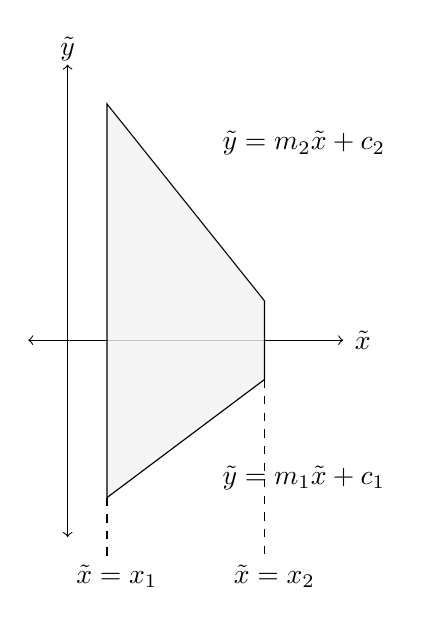
\begin{tikzpicture}[scale=0.5]
	\coordinate(negx) at (-1,0);
	\coordinate(posx) at (\lim+2,0);
	\coordinate(negy) at (0,-5);
	\coordinate(posy) at (0,7);
	
	\coordinate(TL) at (1,6);
	\coordinate(BL) at (1,-4);
	\coordinate(TR) at (\lim,1);
	\coordinate(BR) at (\lim,-1);
	
	\draw[<->] (negx) -- (posx);
	\draw[<->] (negy) -- (posy);
	\filldraw[fill=black!5, fill opacity=0.8] (BL) -- (BR) -- (TR) -- (TL) -- cycle;
	
	\draw[dashed] (BL) -- (1,-5.5);
	\node(x1) at (1.25,-6) {\(\tilde{x} = x_1\)};
	\draw[dashed] (BR) -- (\lim,-5.5);
	\node(x2) at (\lim+0.25,-6) {\(\tilde{x} = x_2\)};
	\node(m1c1) at (6,-3.5) {\(\tilde{y}=m_1\tilde{x}+c_1\)};
	\node(m2c2) at (6,5) {\(\tilde{y}=m_2\tilde{x}+c_2\)};
	\node(x) at (\lim+2.5,0) {\(\tilde{x}\)};
	\node(y) at (0,7.4) {\(\tilde{y}\)};
\end{tikzpicture}
	\caption{A trapezial surface parallel to the \(XY\)-plane. It has two parallel edges, \(x = x_1\) and \(x = x_2\), and two nonparallel edges joining them, \(y = m_1x+c_1\) and \(y = m_2x+c_2\).}
	\label{fig:p3trapezium}
\end{figure}

\subsection{Rectangular faces}\label{sec:p3rectFaces}
The field solution for the two rectangular faces is a simplified case of the trapezium. Both rectangular surfaces are already parallel to the \(XY\)-plane, and two edges parallel to the \(y\)-axis, so no rotation is necessary. Since two edges are parallel to the \(x\)-axis, \(m_p = 0\) and Equation (\ref{eqn:p3fieldequation}) is simplified. This simplification is equivalent to the expressions seen in studies on cuboidal magnets \cite{Akoun1984,Ravaud2009a}. The point \(\mathbf{x}\) and geometric parameters can be substituted into Equation (\ref{eqn:p3fieldequation}) to obtain the magnetic field for each of the rectangular surfaces,
\begin{align}
\mathbf{B}_{\text{rect,}i} = \mathbf{B}\left(\mathbf{x}\right) \text{.}
\end{align}

\subsection{Trapezial faces}\label{sec:p3trapFaces}
The fields produced by the four trapezial surface are more difficult to evaluate than those produced by the rectangular surfaces since they require rotation and \(m_p \neq 0\) in general. However, since each of the four trapezia have normal vectors orthogonal to either the \(x\)- or \(y\)-axes, the rotation matrices are simple. If the trapezia are numbered as shown in Figure \ref{fig:p3numberedTrapezia}, then the rotation matrices corresponding to each trapezium are given by
\begin{figure}
	\centering
	\def\lim{5}

\tdplotsetmaincoords{0}{0}
\begin{tikzpicture}[scale=0.115,tdplot_main_coords]

% Define coordinates:
\coordinate(ppb) at (15,20,-20);
\coordinate(pnb) at (15,-20,-20);
\coordinate(nnb) at (-15,-20,-20);
\coordinate(npb) at (-15,20,-20);
\coordinate(ppt) at (5,10,0);
\coordinate(pnt) at (5,-10,0);
\coordinate(nnt) at (-5,-10,0);
\coordinate(npt) at (-5,10,0);

% Draw shape:
\draw (ppt) -- (pnt) -- (nnt) -- (npt) -- cycle;
\draw (ppb) -- (pnb) -- (nnb) -- (npb) -- cycle;
\draw (ppt) -- (ppb);
\draw (pnt) -- (pnb);
\draw (nnt) -- (nnb);
\draw (npt) -- (npb);

% Draw some lines of symmetry
\draw[dashed,black!30] (-20,0,0) -- (20,0,0);
\draw[dashed,black!30] (0,-25,0) -- (0,25,0);

% Number the trapezia:
\node[circle,draw,fill=white](1) at (11,0,0) {1};
\node[circle,draw,fill=white](2) at (0,16,0) {2};
\node[circle,draw,fill=white](3) at (-11,0,0) {3};
\node[circle,draw,fill=white](4) at (0,-16,0) {4};

% Axes:
\draw[->] (0,0,0) -- (\lim,0,0);
\draw[->] (0,0,0) -- (0,\lim,0);
%\draw[->] (0,0,0) -- (0,0,\lim);
\node(xaxis) at (\lim+2,0,0) {\(x\)};
\node(yaxis) at (0,\lim+2,0) {\(y\)};
%\node(zaxis) at (0,0,\lim+2) {\(z\)};



\end{tikzpicture}
	\caption{A pyramid frustum as viewed from the positive \(z\)-axis with the four angled surfaces numbered.}
	\label{fig:p3numberedTrapezia}
\end{figure}
\begin{align}
\begin{split}
R_1 &= \begin{bmatrix}
n_z & 0 & n_x \\
0 & 1 & 0 \\
-n_x & 0 & n_z
\end{bmatrix} \text{,}
\quad
R_2 = \begin{bmatrix}
0 & n_z & -n_y \\
-1 & 0 & 0 \\
0 & n_y & n_z
\end{bmatrix} \text{,} \\[3mm]
R_3 &= \begin{bmatrix}
n_z & 0 & -n_x \\
0 & 1 & 0 \\
n_x & 0 & n_z
\end{bmatrix} \text{,}
\quad
R_4 = \begin{bmatrix}
0 & -1 & 0 \\
n_z & 0 & n_y \\
-n_y & 0 & n_z
\end{bmatrix} \text{,}
\end{split}
\end{align}
where \(\hat{\mathbf{n}} = \left[ n_x, n_y, n_z \right]\) is the outward-facing unit normal vector of each trapezium.

The rotation matrix \(R_j\) defines a temporary coordinate system \(\left( \tilde{x}, \tilde{y}, \tilde{z} \right)\) in which the trapezium is parallel to the \(\tilde{X}\tilde{Y}\)-plane, allowing the use of Equation (\ref{eqn:p3fieldequation}). In this new coordinate system, the field point is given by \(\mathbf{x} R_j\) and the vertices of the trapezium in the new coordinate system can be similarly found by postmultiplying by \(R_j\). Once the field is calculated in the new coordinate system, it can be transformed back to the original coordinate system by postmultiplying by \(R_j^{-1}\). Thus, the field contribution of each trapezium is given by
\begin{equation}
\mathbf{B}_{\text{trap,}j} = \mathbf{B}\left( \mathbf{x} R_j \right) R_j^{-1} \text{.}
\end{equation}